\documentclass{article}
\usepackage[utf8x]{inputenc}
\usepackage[russianb]{babel}
\usepackage[usenames]{color}
\usepackage{vmargin}
\usepackage{ amssymb }
\usepackage{listings}
\usepackage[linesnumbered,boxed]{algorithm2e}
\usepackage{graphicx}
\usepackage{amsthm}
\usepackage{setspace}
\usepackage{indentfirst}
\usepackage[noend]{algorithmic}
\onehalfspacing
\setpapersize{A4}
\setmarginsrb{3cm}{2cm}{3cm}{2cm}{0pt}{0mm}{0pt}{13mm}
\sloppy
\renewcommand\contentsname{Оглавление}
\renewcommand{\labelenumi}{\theenumi)}

\begin{document}

\null\hfill\begin{tabular}[t]{l@{}}
	\textit{Kirill Zuev}
\end{tabular}

\begin{center}
	\textbf{Home assignment № 2}
\end{center}

\textbf{Task 1.}

Mark the names of air companies with $g_i$ ($i = 1, \dots, 13$) and the names of regions with $m_j$ ($j = 1, \dots, 9$). I wrote a Haskell program \textit{FormalConcepts.hs} to find all formal concepts:

\begin{enumerate}
	\item {$A = \{g_1,g_2,g_3,g_4,g_5,g_6,g_7,g_8,g_9,g_{10},g_{11},g_{12},g_{13}\},~B = \varnothing $}
	\item {$A = \{g_1,g_2,g_3,g_5,g_6,g_7,g_9,g_{10},g_{11},g_{12},g_{13}\},~B = \{m_2\}$}
	\item {$A = \{g_1,g_2,g_3,g_4,g_5,g_7,g_9,g_{10},g_{11},g_{12},g_{13}\},~B = \{m_4\}$}
	\item {$A = \{g_1,g_2,g_3,g_5,g_7,g_8,g_9,g_{10},g_{11},g_{12},g_{13}\},~B = \{m_9\}$}
	\item {$A = \{g_1,g_7,g_8,g_9,g_{11},g_{12},g_{13}\},~B = \{m_1,m_9\}$}
	\item {$A = \{g_1,g_5,g_7,g_8,g_{10},g_{12}\},~B = \{m_3,m_9\}$}
	\item {$A = \{g_1,g_2,g_3,g_5,g_7,g_9,g_{10},g_{11},g_{12},g_{13}\},~B = \{m_2,m_4,m_9\}$}
	\item {$A = \{g_1,g_7,g_9,g_{11},g_{12},g_{13}\},~B = \{m_1,m_2,m_4,m_9\}$}
	\item {$A = \{g_1,g_5,g_7,g_{10},g_{12}\},~B = \{m_2,m_3,m_4,m_9\}$}
	\item {$A = \{g_1,g_5,g_7,g_{10}\},~B = \{m_2,m_3,m_4,m_5,m_9\}$}
	\item {$A = \{g_5,g_7,g_9,g_{10},g_{13}\},~B = \{m_2,m_4,m_6,m_9\}$}
	\item {$A = \{g_7,g_9,g_13\},~B = \{m_1,m_2,m_4,m_6,m_9\}$}
	\item {$A = \{g_5,g_7,g_{10}\},~B = \{m_2,m_3,m_4,m_5,m_6,m_9\}$}
	\item {$A = \{g_1,g_7,g_8,g_{12},g_{13}\},~B = \{m_1,m_7,m_9\}$}
	\item {$A = \{g_1,g_7,g_8,g_{12}\},~B = \{m_1,m_3,m_7,m_9\}$}
	\item {$A = \{g_1,g_7,g_{12},g_{13}\},~B = \{m_1,m_2,m_4,m_7,m_9\}$}
	\item {$A = \{g_1,g_7,g_{12}\},~B = \{m_1,m_2,m_3,m_4,m_7,m_9\}$}
	\item {$A = \{g_1,g_7\},~B = \{m_1,m_2,m_3,m_4,m_5,m_7,m_9\}$}
	\item {$A = \{g_7,g_{13}\},~B = \{m_1,m_2,m_4,m_6,m_7,m_9\}$}
	\item {$A = \{g_7\},~B = \{m_1,m_2,m_3,m_4,m_5,m_6,m_7,m_9\}$}
	\item {$A = \{g_1,g_8,g_{11},g_{12}\},~B = \{m_1,m_8,m_9\}$}
	\item {$A = \{g_1,g_{11},g_{12}\},~B = \{m_1,m_2,m_4,m_8,m_9\}$}
	\item {$A = \{g_1,g_8,g_{12}\},~B = \{m_1,m_3,m_7,m_8,m_9\}$}
	\item {$A = \{g_1,g_{12}\},~B = \{m_1,m_2,m_3,m_4,m_7,m_8,m_9\}$}
	\item {$A = \{g_1\},~B = \{m_1,m_2,m_3,m_4,m_5,m_7,m_8,m_9\}$}
	\item {$A = \varnothing,~B = \{m_1,m_2,m_3,m_4,m_5,m_6,m_7,m_8,m_9\}$}
\end{enumerate}

\textbf{Task 2.}

\begin{figure}[h]
	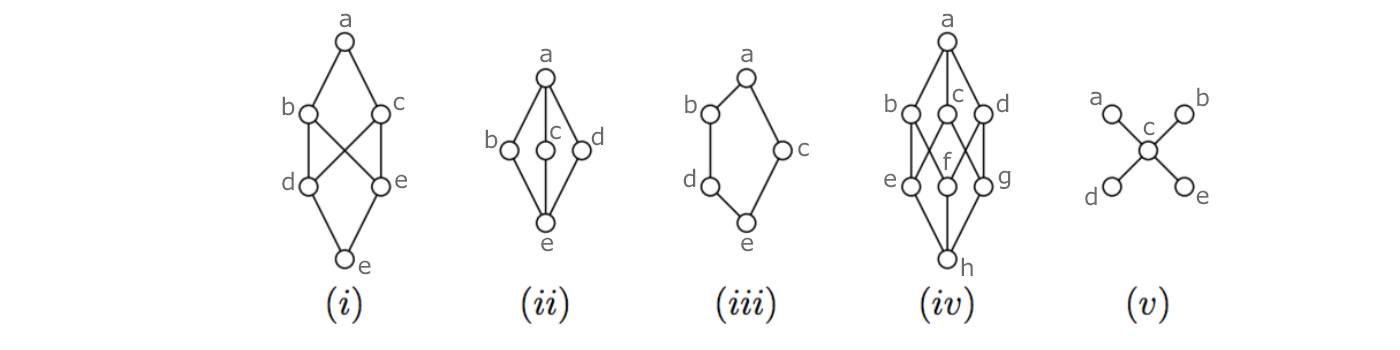
\includegraphics[width=\linewidth]{2.png}
\end{figure}

$(i)$ $\nexists d \lor e$ $\Rightarrow$ It is not a lattice.\\

$(ii)$ Diamond is a lattice. And it is complete because all finite lattices are complete.

$a \lor x = a$ ($x = b, \dots e$), $b \lor c = b \lor d = c \lor d = a$, $e \lor x = x$ ($x = b, \dots, d$)

$e \land x = e$ ($x = a, \dots d$), $b \land c = b \land d = c \land d = e$, $a \land x = x$ ($x = b, \dots, d$)\\

$(iii)$ Pentagon is a lattice. And it is complete because all finite lattices are complete.

$a \lor x = a$ ($x = b, \dots e$), $b \lor c = c \lor d = a$, $b \lor d = b$, $e \lor x = x$ ($x = b, \dots, d$)

$e \land x = e$ ($x = a, \dots d$), $b \land c = c \land d = e$, $b \land d = d$, $a \land x = x$ ($x = b, \dots, d$)\\

$(iv)$ Boolean cube is a lattice because all pairs have supremum and infimum. And it is complete because all finite lattices are complete.\\

$(v)$ $\nexists a \lor b$ $\Rightarrow$ It is not a lattice.\\

\textbf{Task 3.}

$(L, \leq)$ is a lattice with infimum and supremum defined as usual.

$\forall x,y \in L:$\\

a) $x \lor x = sup\{x, x\} = sup\{x\} = x$\\

b) $x \lor (x \land y) = sup\{x, inf\{x,y\}\}$

$y \leq x \Rightarrow sup\{x, inf\{x,y\}\} = sup\{x,y\} = x$

$x \leq y \Rightarrow sup\{x, inf\{x,y\}\} = sup\{x,x\} = x$\\

c) $x \lor y = sup\{x, y\} = sup\{y, x\} = y \lor x$

 \end{document}